\documentclass[11pt]{article}
\usepackage{lingmacros}
\usepackage{tree-dvips}
\usepackage{graphicx}
\usepackage{hyperref}
\usepackage[utf8]{inputenc}
\usepackage[french]{babel}
\usepackage{listings}
\usepackage{color}
\usepackage[T1]{fontenc}
\usepackage[a4paper, total={7in, 10in}]{geometry}

\definecolor{codegreen}{rgb}{0,0.6,0}
\definecolor{codegray}{rgb}{0.5,0.5,0.5}
\definecolor{codepurple}{rgb}{0.58,0,0.82}
\definecolor{backcolour}{rgb}{0.95,0.95,0.92}

\lstdefinestyle{mystyle}{
    backgroundcolor=\color{backcolour},   
    commentstyle=\color{codegreen},
    keywordstyle=\color{magenta},
    numberstyle=\tiny\color{codegray},
    stringstyle=\color{codepurple},
    basicstyle=\ttfamily\footnotesize,
    breakatwhitespace=false,         
    breaklines=true,                 
    captionpos=b,                    
    keepspaces=true,                 
    numbers=left,                    
    numbersep=5pt,                  
    showspaces=false,                
    showstringspaces=false,
    showtabs=false,                  
    tabsize=2
}

\lstset{style=mystyle}

\author{Esteban Becker}
\date{05/05/2023}
\title{TP 2 HTTPS CONNEXION}

\begin{document}

\maketitle

\section{Vérification du serveur http}

Dans le code nous avons modifié la ligne suivante :

\begin{lstlisting}[language=Python]
    # definir le message secret
    SECRET_MESSAGE = "Je_suis_un_super_mot_de_passe" # A modifier
    app = Flask(__name__)
\end{lstlisting}

\begin{figure}[!htb]
    \centering
    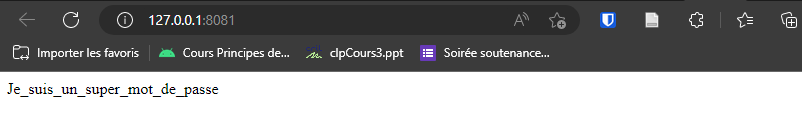
\includegraphics[width=\textwidth]{images/Navigateur_premier_mdp.png}
    \caption{Capture d'écran du Navigateur}
    \label{fig:1navigateur}
\end{figure}

\begin{figure}[!htb]
    \centering
    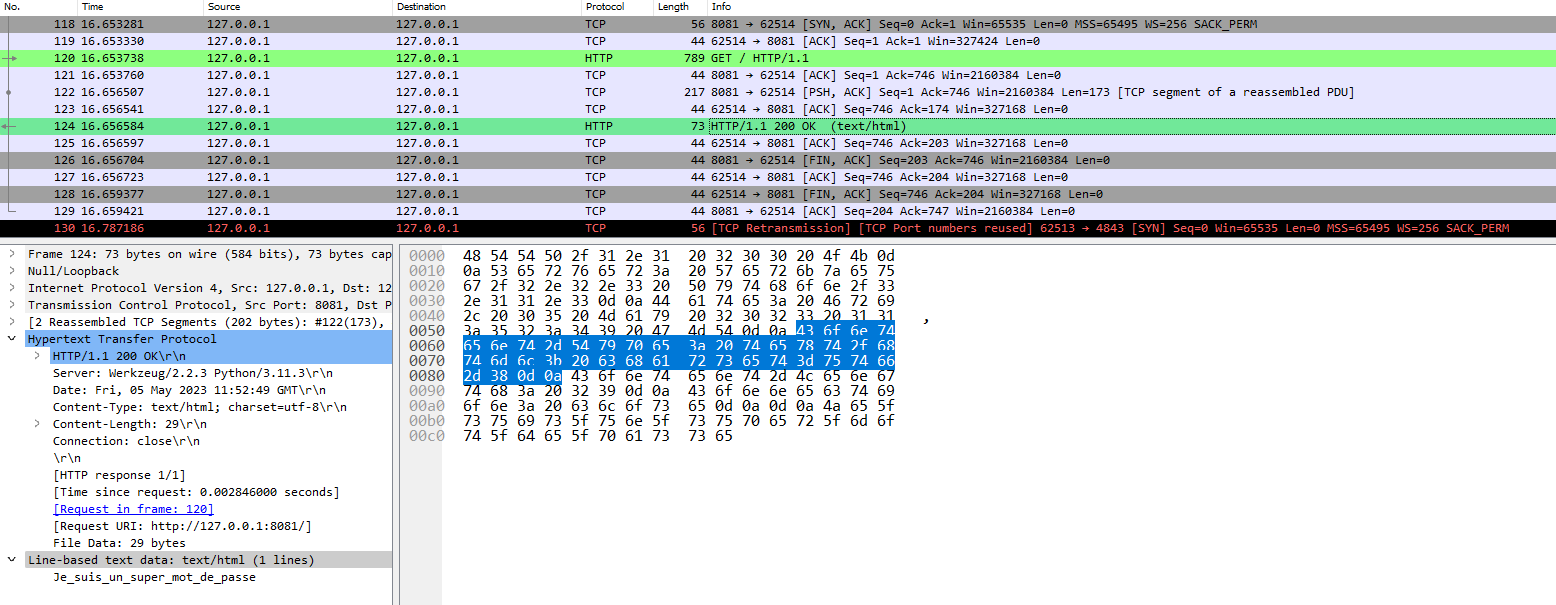
\includegraphics[width=\textwidth]{images/Wireshark_premier_mdp.png}
    \caption{Capture d'écran de Wireshark}
    \label{fig:1Wireshark}
\end{figure}


Ainsi dans a capture Wireshark nous avons sélectionné l'interface du réseau local de la machine, une fois la capture lancé, nous recherchons les emplacements où le protocole utilisé est HTTP.
Deux paquets sont alors détectés. Il y a le paquet get, qui est celui de demande de la page, ensuite, il y a le paquet de réponse.
Dans la réponse on peut voir que le mot de passe est en clair, ce qui est une faille de sécurité.
Le mot de passe est dans la requête hexadécimale à droite, mais dans le panel de gauche, Wireshark nous donne la traduction en ASCII, ce qui correspond au mot de passe défini dans le code python.

\section{Génération du certificat de l'autorité de certification}

Afin de faire fonctionner le code, il a fallu mettre les bons paramètres dans chaque fonction.

Pour le certificat, les paramètres sont les suivants :

\begin{lstlisting}[language=Python]

    CA_PASSWORD = "XsFa$qN2H9bq^&Y@osMdR5Nqn6T2oDghC&Zij*xgSzXW!7m*hYDToVZukWFKVsaZo9hjSaprUftufpimcSdvhg2k!BwcZp5E4LjGoFEe$QHkLv65ozk*MGee8#BFfsHL"
    CA_CONFIGURATION = Configuration("FR", "Territoire de Belfort", "Belfort", "EstebanBecker_CA", "localhost") 
    
\end{lstlisting}

Le mot de passe a été généré en utilisant un générateur aléatoire de mots de passes.

La clé publique est la suivante :

\begin{figure}[!htb]
    \centering
    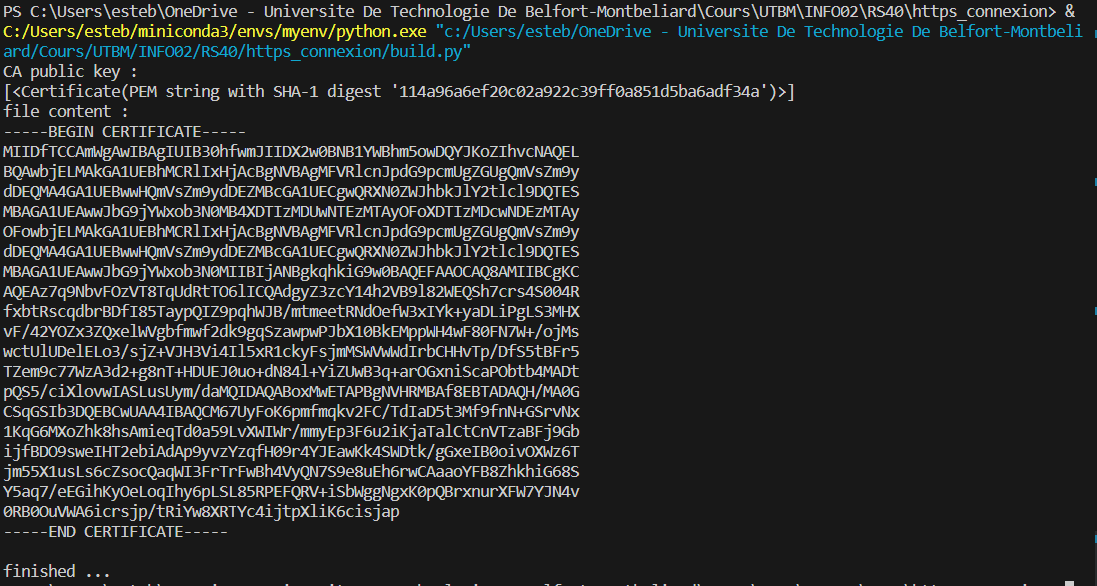
\includegraphics[width=\textwidth]{images/Certificat.png}
    \caption{Capture d'écran de Wireshark}
    \label{fig:Certificat}
\end{figure}

\end{document}